\section{Phân tích các yếu tố ảnh hưởng đến Quyết định Nghỉ việc (HR Employee Attrition)}
\label{sec:hr-attrition}

\subsection{Bối cảnh, câu hỏi nghiên cứu và phạm vi phân tích}

Nghỉ việc tự nguyện làm phát sinh chi phí tuyển dụng, đào tạo thay thế,
gián đoạn vận hành và thất thoát tri thức tổ chức. Vì vậy, bài toán của
phần này không chỉ là dự đoán một nhân viên có nghỉ việc hay không, mà
còn nhằm xác định các nhóm yếu tố có liên hệ mạnh với rủi ro nghỉ việc
để hỗ trợ bộ phận nhân sự ưu tiên can thiệp.

Ba mục tiêu cụ thể được đặt ra như sau:

\begin{enumerate}
  \item \textbf{Khám phá dữ liệu:} mô tả chân dung nhóm nghỉ việc và
  đánh giá vai trò của thu nhập, tuổi, phòng ban, vị trí, làm thêm giờ,
  mức độ hài lòng và lịch sử công tác;
  \item \textbf{Xây dựng mô hình dự báo:} so sánh hồi quy logistic theo
  hai nhóm biến có chủ đích với hồi quy logistic phạt LASSO sử dụng toàn bộ thông tin;
  \item \textbf{Chuyển kết quả thành hàm ý quản trị:} đề xuất cơ chế
  cảnh báo sớm và chính sách giữ chân nhân viên phù hợp với các nhóm rủi ro cao.
\end{enumerate}

Biến phản hồi là \texttt{Attrition}, nhận hai giá trị \texttt{Yes}
(đã nghỉ việc) và \texttt{No} (còn làm việc). Do đây là biến nhị phân,
bài toán thuộc lớp bài toán phân loại có giám sát. Các kết quả trong
phần này phản ánh \emph{mối liên hệ dự báo} trong bộ dữ liệu mô phỏng,
không tự thân chứng minh quan hệ nhân quả. Chẳng hạn, hệ số dương của
\texttt{OverTime} không đủ để kết luận làm thêm giờ là nguyên nhân duy
nhất gây nghỉ việc nếu chưa kiểm soát thiết kế nghiên cứu và các yếu tố
gây nhiễu.

\subsection{Bộ dữ liệu và hệ thống biến}

\subsubsection{Nguồn gốc và đơn vị quan sát}

Bộ dữ liệu \texttt{WA\_Fn-UseC\_-HR-Employee-Attrition.csv}, thường
được biết đến với tên \emph{IBM HR Analytics Employee Attrition \&
Performance}, là dữ liệu mô phỏng phục vụ đào tạo và thực hành phân tích nhân sự. Dữ liệu gồm \textbf{1.470 nhân viên và 35 biến}. Vì là dữ liệu mô phỏng, kết quả phù hợp để minh họa quy trình mô hình hóa nhưng không nên được khái quát trực tiếp cho một doanh nghiệp cụ thể nếu chưa hiệu chỉnh và kiểm định trên dữ liệu thực tế của doanh nghiệp đó.
Các thống kê mô tả được tính trên bộ dữ liệu gốc trước khi capping và
chuẩn hóa \cite{ibm_attrition_data}.

\subsubsection{Các nhóm biến giải thích}

Sau biến phản hồi, các biến giải thích được tổ chức theo năm nhóm nội
dung. Cách phân nhóm này giúp diễn giải mô hình theo cơ chế quản trị,
thay vì xem mỗi cột dữ liệu như một thuộc tính rời rạc.

\begin{longtable}{p{0.19\linewidth}p{0.35\linewidth}p{0.38\linewidth}}
\caption{Các nhóm biến trong bộ dữ liệu nghỉ việc.}\label{tab:hr-variable-groups}\\
\toprule
Nhóm & Biến tiêu biểu & Nội dung đo lường\\
\midrule
\endfirsthead
\toprule
Nhóm & Biến tiêu biểu & Nội dung đo lường\\
\midrule
\endhead
Thông tin cá nhân & \texttt{Age}, \texttt{Gender},
\texttt{MaritalStatus}, \texttt{Education},
\texttt{EducationField}, \texttt{DistanceFromHome} & Tuổi, giới tính,
tình trạng hôn nhân, học vấn, chuyên ngành và khoảng cách đi làm.\\
Vai trò và công việc & \texttt{Department}, \texttt{JobRole},
\texttt{JobLevel}, \texttt{BusinessTravel}, \texttt{JobInvolvement} &
Phòng ban, chức danh, cấp bậc, tần suất công tác và mức độ tham gia công
việc.\\
Thu nhập và đãi ngộ & \texttt{MonthlyIncome},
\texttt{PercentSalaryHike}, \texttt{StockOptionLevel},
\texttt{OverTime}, \texttt{DailyRate}, \texttt{HourlyRate},
\texttt{MonthlyRate} & Thu nhập, tăng lương, quyền chọn cổ phiếu, làm
thêm giờ và các chỉ số thù lao.\\
Đánh giá và hài lòng & \texttt{EnvironmentSatisfaction},
\texttt{JobSatisfaction}, \texttt{RelationshipSatisfaction},
\texttt{WorkLifeBalance}, \texttt{PerformanceRating} & Các thang đo từ
1 (thấp) đến 4 (rất cao), riêng đánh giá hiệu suất chủ yếu nhận mức 3--4.\\
Lịch sử và thâm niên & \texttt{TotalWorkingYears},
\texttt{NumCompaniesWorked}, \texttt{YearsAtCompany},
\texttt{YearsInCurrentRole}, \texttt{YearsSinceLastPromotion},
\texttt{YearsWithCurrManager}, \texttt{TrainingTimesLastYear} & Kinh
nghiệm, số công ty từng làm, thâm niên, thời gian ở vai trò hiện tại,
thăng tiến, quan hệ với quản lý và đào tạo.\\
\bottomrule
\end{longtable}

Bốn biến cần loại khỏi tập dự báo gồm \texttt{EmployeeCount},
\texttt{Over18} và \texttt{StandardHours}, do chỉ có một giá trị duy
nhất, cùng \texttt{EmployeeNumber}, do đây là mã định danh. Biến phương
sai bằng 0 không thể giải thích sự khác biệt giữa các quan sát; mã định
danh có thể khiến mô hình học thuộc mẫu mà không mang ý nghĩa nghiệp vụ.

\subsection{Khám phá và tiền xử lý dữ liệu}

\subsubsection{Khám phá dữ liệu ban đầu và thống kê mô tả}

Kết quả đọc dữ liệu xác nhận kích thước \(1470\times35\). Ba biến
\texttt{EmployeeCount}, \texttt{Over18} và \texttt{StandardHours} có
phương sai bằng 0; \texttt{EmployeeNumber} là định danh nên được loại.
Sau bước này, dữ liệu không có giá trị khuyết (0 giá trị
\texttt{NA}). Vì vậy, không thực hiện điền khuyết. Quyết định này tránh
đưa thêm sai số và giả định không cần thiết từ một phương pháp gán thay
thế.

Toàn bộ 23 biến số còn lại sau khi loại mã định danh và các biến phương
sai bằng 0 được tóm tắt trong Bảng \ref{tab:hr-descriptive}. Báo cáo sử
dụng bảy đại lượng: nhỏ nhất, tứ phân vị thứ nhất \(Q_1\), trung vị
\(Q_2\), tứ phân vị thứ ba \(Q_3\), lớn nhất, trung bình và độ lệch
chuẩn mẫu. Ba tứ phân vị giúp mô tả vị trí và độ phân tán mà ít nhạy với
giá trị cực đoan hơn trung bình và độ lệch chuẩn.

\begin{landscape}
\scriptsize
\begin{longtable}{>{\raggedright\arraybackslash}p{0.27\linewidth}rrrrrrr}
\caption{Thống kê mô tả toàn bộ biến định lượng sau khi loại biến hằng
và biến định danh.}\label{tab:hr-descriptive}\\
\toprule
Biến & Min & \(Q_1\) & Median & \(Q_3\) & Max & Mean & SD\\
\midrule
\endfirsthead
\toprule
Biến & Min & \(Q_1\) & Median & \(Q_3\) & Max & Mean & SD\\
\midrule
\endhead
\texttt{Age} & 18 & 30 & 36 & 43 & 60 & 36,92 & 9,14\\
\texttt{DailyRate} & 102 & 465 & 802 & 1.157 & 1.499 & 802,49 & 403,51\\
\texttt{DistanceFromHome} & 1 & 2 & 7 & 14 & 29 & 9,19 & 8,11\\
\texttt{Education} & 1 & 2 & 3 & 4 & 5 & 2,91 & 1,02\\
\texttt{EnvironmentSatisfaction} & 1 & 2 & 3 & 4 & 4 & 2,72 & 1,09\\
\texttt{HourlyRate} & 30 & 48 & 66 & 83,75 & 100 & 65,89 & 20,33\\
\texttt{JobInvolvement} & 1 & 2 & 3 & 3 & 4 & 2,73 & 0,71\\
\texttt{JobLevel} & 1 & 1 & 2 & 3 & 5 & 2,06 & 1,11\\
\texttt{JobSatisfaction} & 1 & 2 & 3 & 4 & 4 & 2,73 & 1,10\\
\texttt{MonthlyIncome} & 1.009 & 2.911 & 4.919 & 8.379 & 19.999 & 6.502,93 & 4.707,96\\
\texttt{MonthlyRate} & 2.094 & 8.047 & 14.235,5 & 20.461,5 & 26.999 & 14.313,10 & 7.117,79\\
\texttt{NumCompaniesWorked} & 0 & 1 & 2 & 4 & 9 & 2,69 & 2,50\\
\texttt{PercentSalaryHike} & 11 & 12 & 14 & 18 & 25 & 15,21 & 3,66\\
\texttt{PerformanceRating} & 3 & 3 & 3 & 3 & 4 & 3,15 & 0,36\\
\texttt{RelationshipSatisfaction} & 1 & 2 & 3 & 4 & 4 & 2,71 & 1,08\\
\texttt{StockOptionLevel} & 0 & 0 & 1 & 1 & 3 & 0,79 & 0,85\\
\texttt{TotalWorkingYears} & 0 & 6 & 10 & 15 & 40 & 11,28 & 7,78\\
\texttt{TrainingTimesLastYear} & 0 & 2 & 3 & 3 & 6 & 2,80 & 1,29\\
\texttt{WorkLifeBalance} & 1 & 2 & 3 & 3 & 4 & 2,76 & 0,71\\
\texttt{YearsAtCompany} & 0 & 3 & 5 & 9 & 40 & 7,01 & 6,13\\
\texttt{YearsInCurrentRole} & 0 & 2 & 3 & 7 & 18 & 4,23 & 3,62\\
\texttt{YearsSinceLastPromotion} & 0 & 0 & 1 & 3 & 15 & 2,19 & 3,22\\
\texttt{YearsWithCurrManager} & 0 & 2 & 3 & 7 & 17 & 4,12 & 3,57\\
\bottomrule
\end{longtable}
\end{landscape}

Các thống kê cho thấy \texttt{MonthlyIncome} lệch phải rõ: trung bình
6.502,93 USD cao hơn trung vị 4.919 USD, đồng thời \(Q_3=8.379\) USD
nhưng giá trị lớn nhất đạt 19.999 USD. \texttt{MonthlyRate} có độ phân
tán rất lớn nhưng trung bình gần trung vị hơn. Các biến thâm niên cũng
lệch phải: \texttt{YearsAtCompany} có trung bình 7,01 năm, trung vị 5
năm và \(Q_3=9\) năm; \texttt{YearsSinceLastPromotion} có trung vị chỉ
1 năm nhưng giá trị lớn nhất là 15 năm.

Các biến \texttt{Education}, \texttt{EnvironmentSatisfaction},
\texttt{JobInvolvement}, \texttt{JobLevel}, \texttt{JobSatisfaction},
\texttt{PerformanceRating}, \texttt{RelationshipSatisfaction},
\texttt{StockOptionLevel} và \texttt{WorkLifeBalance} được lưu dưới
dạng số nhưng bản chất là thang thứ bậc. Trung bình và độ lệch chuẩn của
chúng được báo cáo để mô tả, song khi diễn giải cần chú ý khoảng cách
giữa hai mức liên tiếp không nhất thiết phản ánh một lượng thay đổi hoàn
toàn bằng nhau.

Cỡ mẫu lớn không đồng nghĩa mọi biến đều phân phối chuẩn và cũng không
tự động bảo đảm mọi kiểm định tham số là hợp lệ. Định lý giới hạn trung
tâm chủ yếu mô tả phân phối của một số thống kê mẫu trong những điều
kiện nhất định; do đó, lựa chọn kiểm định vẫn phải dựa trên dạng biến,
phân phối, phương sai và câu hỏi nghiên cứu.

\subsubsection{Tiền xử lý dữ liệu}

\paragraph{Xử lý thu nhập lệch phải và ngoại lệ.}

Áp dụng quy tắc \(1{,}5\times IQR\) để xác định biên. Đây là
\emph{inner fence} do Tukey đề xuất trong phân tích khám phá dữ liệu
\cite{tukey1977}. Quy tắc này được lựa chọn vì \texttt{MonthlyIncome}
có phân phối lệch phải rõ rệt; khi đó, ngưỡng dựa trên trung bình và độ
lệch chuẩn như \(\bar{x}\pm3s\) dễ bị chính các giá trị lớn kéo lệch.
Ngược lại, \(Q_1\), \(Q_3\) và IQR là các thống kê thứ hạng có tính
kháng nhiễu, ít nhạy với giá trị cực đoan và không đòi hỏi giả định phân
phối chuẩn. Hệ số 1,5 là quy ước khám phá tạo sự cân bằng giữa việc nhận
diện điểm xa vùng dữ liệu trung tâm và tránh gắn nhãn quá nhiều biến
động tự nhiên là ngoại lệ; đây không phải bằng chứng rằng quan sát vượt
biên là dữ liệu sai.

\[
L=Q_1-1{,}5IQR,\qquad U=Q_3+1{,}5IQR,
\]

Sau đó, \texttt{MonthlyIncome} được winsor hóa: giá trị thấp hơn \(L\) được
đưa về \(L\), giá trị cao hơn \(U\) được đưa về \(U\). Biến mới được đặt
tên \texttt{MonthlyIncome\_Capped}. Capping thay vì xóa dòng giúp bảo
toàn cỡ mẫu và giảm ảnh hưởng của các giá trị cực lớn lên quá trình ước
lượng. Do mức thu nhập cao vẫn có thể hợp lệ đối với quản lý cấp cao,
thống kê mô tả và kiểm định Wilcoxon tiếp tục dùng thu nhập gốc; biến
capping chỉ được dùng như đặc trưng kỹ thuật trong mô hình. Cách trình
bày song song này tránh đồng nhất ``bất thường theo phân phối'' với
``sai số đo lường'' và tạo cơ sở cho phân tích độ nhạy.

\paragraph{Mã hóa và chuẩn hóa.}

Các biến ký tự được chuyển sang biến phân loại; khi lập ma trận thiết
kế, mỗi mức của biến phân loại được mã hóa bằng biến giả. Tuổi và thu
nhập sau capping được chuẩn hóa theo

\[
z_i=\frac{x_i-\bar{x}}{s_x}.
\]

Chuẩn hóa không bắt buộc đối với hồi quy logistic không phạt, nhưng cần
thiết với LASSO vì hình phạt \(L_1\) tác động trực tiếp lên độ lớn hệ số.
Nếu thang đo khác nhau, biến có đơn vị lớn có thể bị phạt không công
bằng. Hệ số của \texttt{Age\_scaled} vì thế được hiểu theo một độ lệch
chuẩn tuổi, thay vì một năm tuổi.

Phiên bản báo cáo mới đã điều chỉnh quy trình để tránh rò rỉ dữ liệu:
các biên IQR và tham số chuẩn hóa không còn được ước lượng trên toàn bộ
mẫu mà chỉ được học từ tập huấn luyện. Chi tiết pipeline được trình bày
ở Mục \ref{sec:hr-strict-pipeline}.

\subsubsection{Phân tích khám phá và trực quan hóa}

\paragraph{Phân phối biến phản hồi và hệ quả mất cân bằng lớp.}

Trong 1.470 nhân viên, có 1.233 người ở lại (83,88\%) và 237 người
nghỉ việc (16,12\%); tỷ lệ hai lớp xấp xỉ \(5{,}2:1\).

\begin{figure}[H]
\centering
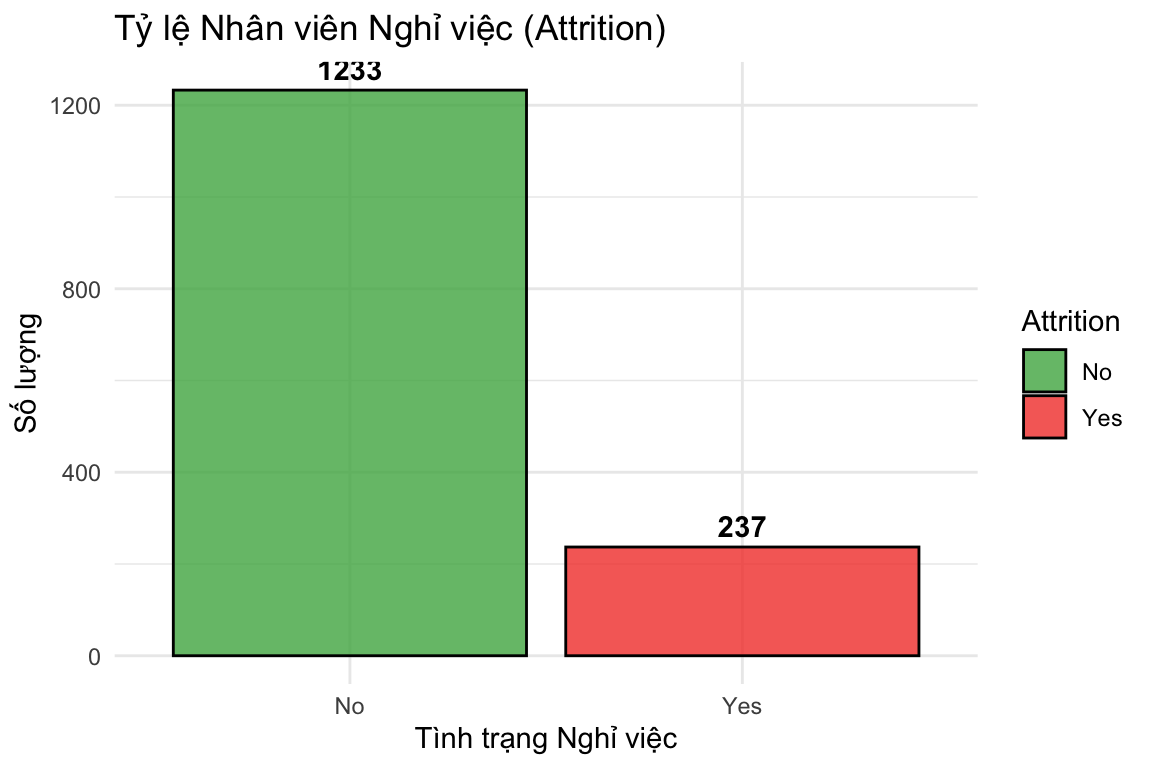
\includegraphics[width=0.78\linewidth]{img/hr-attrition-distribution.png}
\caption{Phân phối tình trạng nghỉ việc trong bộ dữ liệu.}
\label{fig:hr-attrition-distribution}
\end{figure}

Mất cân bằng lớp khiến accuracy dễ gây hiểu lầm: một bộ phân loại luôn
dự báo \texttt{No} đã đạt 83,88\% accuracy nhưng sensitivity đối
với lớp nghỉ việc bằng 0. Vì mục tiêu quản trị là nhận diện người có rủi
ro, báo cáo ưu tiên AUC, sensitivity/recall, precision và F1-score. Các
hướng xử lý có thể gồm trọng số lớp, hạ ngưỡng quyết định, undersampling,
SMOTE hoặc ROSE. Phân tích không tái lấy mẫu trong mô hình chính mà sử
dụng ngưỡng vận hành 0,3; sự đánh đổi của ngưỡng này được đánh giá riêng
ở Mục \ref{sec:hr-threshold}.

\paragraph{Thu nhập và tình trạng nghỉ việc.}

Biểu đồ hộp cho thấy trung vị thu nhập của nhóm ở lại khoảng 5.200
USD/tháng, cao hơn nhóm nghỉ việc khoảng 3.200 USD/tháng. Khoảng tứ phân
vị của nhóm ở lại xấp xỉ 3.200--8.800 USD, trong khi nhóm nghỉ việc tập
trung khoảng 2.400--6.000 USD. Nhóm nghỉ việc vẫn có một số trường hợp
thu nhập 12.000--20.000 USD, vì thế không thể xem mọi mức lương cao là
ngoại lệ sai.

\begin{figure}[H]
\centering
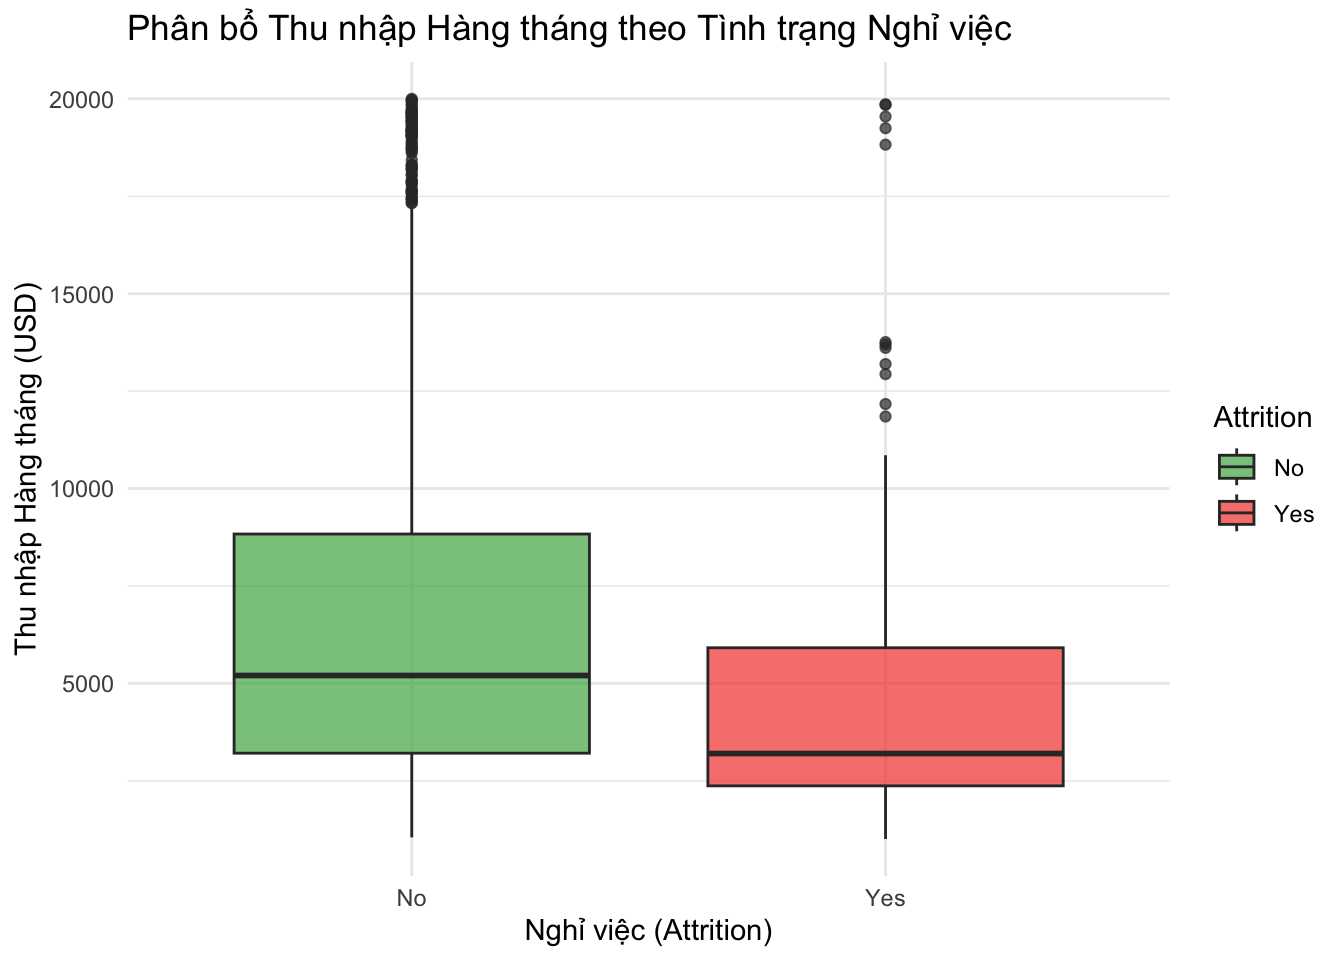
\includegraphics[width=0.82\linewidth]{img/hr-income-by-attrition.png}
\caption{Phân phối thu nhập hàng tháng theo tình trạng nghỉ việc.}
\label{fig:hr-income-attrition}
\end{figure}

Hình \ref{fig:hr-income-attrition} cung cấp bằng chứng mô tả rằng nhóm
nghỉ việc có phân phối thu nhập thấp hơn, nhưng chưa chứng minh tác động
nhân quả của tiền lương. Thu nhập liên hệ chặt với tuổi, cấp bậc, vị trí
và thâm niên; vì vậy, hệ số thu nhập có thể thay đổi khi đưa đồng thời
các biến này vào mô hình đa biến.

\paragraph{Tuổi và tình trạng nghỉ việc.}

Nhóm nghỉ việc có tuổi trung bình khoảng 33--34, thấp hơn nhóm ở lại với số tuổi trung bình khoảng 37--38 tuổi. Mật độ của nhóm nghỉ việc tập trung mạnh ở 28--32
tuổi; từ khoảng 35 tuổi trở lên, mật độ của nhóm ở lại chiếm ưu thế.
Nhận định hợp lý ở đây là tuổi cung cấp tín hiệu dự báo, không phải nhân viên trẻ tất yếu nghỉ việc.

\begin{figure}[H]
\centering
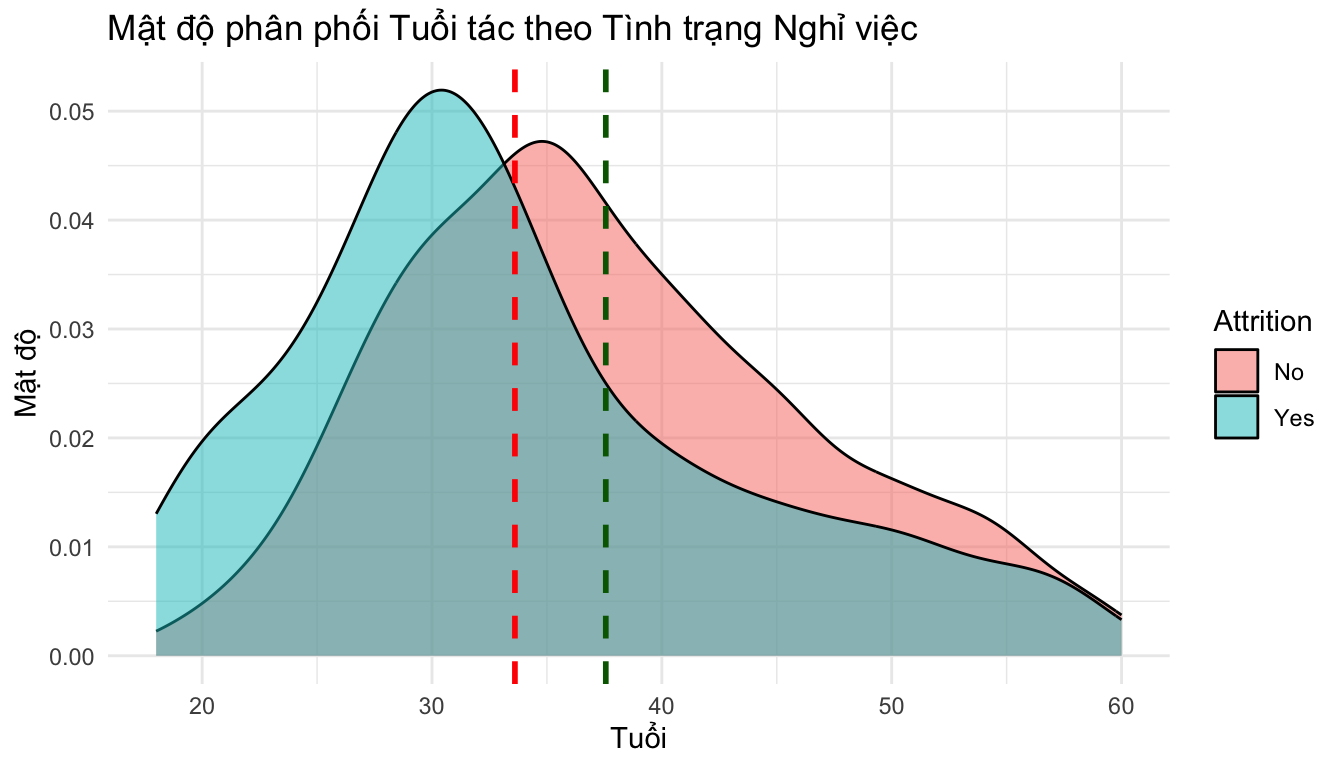
\includegraphics[width=0.84\linewidth]{img/hr-age-density.png}
\caption{Mật độ tuổi theo tình trạng nghỉ việc.}
\label{fig:hr-age-density}
\end{figure}

\subsubsection{Kiểm định thống kê}

\paragraph{Kiểm định phân phối thu nhập.}

Với 237 nhân viên nghỉ việc, kiểm định Shapiro--Wilk cho
\texttt{MonthlyIncome} cho kết quả \(W=0{,}780\),
\(p=1{,}50\times10^{-17}\). Ở mức ý nghĩa 5\%, bác bỏ giả thuyết
phân phối chuẩn. Kết quả này, cùng dạng lệch phải trên biểu đồ, là cơ sở
chọn kiểm định Wilcoxon rank-sum thay cho kiểm định \(t\) hai mẫu trong
phân tích nguồn. Wilcoxon kiểm tra sự dịch chuyển phân phối/thứ hạng;
chỉ diễn giải trực tiếp thành khác biệt trung vị khi hình dạng phân phối
hai nhóm đủ tương đồng.

\paragraph{So sánh thu nhập giữa hai nhóm.}

Kiểm định Wilcoxon cho kết quả \(W=191600\),
\(p=2{,}953\times10^{-14}\). Do đó, bác bỏ giả thuyết không có khác biệt
phân phối thu nhập giữa hai nhóm. Kết quả củng cố bằng chứng EDA rằng
nhân viên nghỉ việc thường nằm ở phân khúc thu nhập thấp hơn. File nguồn
có một chỗ ghi \(p<2{,}2\times10^{-16}\), nhưng đầu ra kiểm định thực tế
là \(2{,}953\times10^{-14}\); báo cáo sử dụng giá trị từ đầu ra tính
toán.

\paragraph{Mối liên hệ giữa phòng ban và nghỉ việc.}

Bảng chéo quan sát được là:

\begin{table}[H]
\centering
\caption{Tình trạng nghỉ việc theo phòng ban.}
\label{tab:hr-department}
\begin{tabular}{lrrr}
\toprule
Phòng ban & Ở lại & Nghỉ việc & Tỷ lệ nghỉ việc\\
\midrule
Human Resources & 51 & 12 & 19,05\%\\
Research \& Development & 828 & 133 & 13,84\%\\
Sales & 354 & 92 & 20,63\%\\
\bottomrule
\end{tabular}
\end{table}

Kiểm định Pearson \(\chi^2\) cho kết quả
\(\chi^2=10{,}796\), \(df=2\), \(p=0{,}004526\). Có bằng chứng về mối
liên hệ giữa phòng ban và tình trạng nghỉ việc. R\&D có số người nghỉ
tuyệt đối lớn nhất do quy mô phòng lớn; Sales có tỷ lệ nghỉ việc cao
nhất. Việc phân biệt số tuyệt đối với tỷ lệ là cần thiết để tránh ưu
tiên sai nhóm can thiệp.

Ba kết quả định hướng ban đầu là: nhóm nghỉ việc trẻ hơn, có phân phối
thu nhập thấp hơn và tỷ lệ nghỉ khác nhau theo phòng ban. Tuy nhiên,
kiểm định đơn biến không kiểm soát yếu tố gây nhiễu và có thể phát sinh
sai lầm loại I nếu thực hiện nhiều kiểm định. Do đó, kết luận cuối cùng
phải dựa thêm trên mô hình đa biến và đánh giá ngoài mẫu.

\subsection{Xây dựng mô hình}

\subsubsection{Chia dữ liệu}

Dữ liệu được chia theo tỷ lệ 70\%/30\% bằng
\texttt{createDataPartition} với \texttt{set.seed(123)}. Đây là cách
chia phân tầng theo \texttt{Attrition}, giúp tỷ lệ nghỉ việc giữa tập
huấn luyện và tập kiểm thử gần nhau. Kết quả gồm 1.030 quan sát huấn
luyện (864 ở lại, 166 nghỉ việc) và 440 quan sát kiểm thử (369 ở lại,
71 nghỉ việc). Tập kiểm thử chỉ được dùng để đánh
giá cuối, nhằm ước lượng khả năng tổng quát hóa trên nhân viên chưa xuất
hiện khi huấn luyện.

\subsubsection{Pipeline tiền xử lý không rò rỉ dữ liệu}
\label{sec:hr-strict-pipeline}

Sau khi chia mẫu, các bước phụ thuộc phân phối dữ liệu được thực hiện
theo nguyên tắc \emph{fit trên train, transform trên train và test}.
Trước hết, \(Q_{1,\mathrm{train}}\), \(Q_{3,\mathrm{train}}\) và
\(IQR_{\mathrm{train}}\) của \texttt{MonthlyIncome} được tính chỉ từ
tập huấn luyện. Hai biên

\[
L_{\mathrm{train}}=Q_{1,\mathrm{train}}-1{,}5IQR_{\mathrm{train}},
\qquad
U_{\mathrm{train}}=Q_{3,\mathrm{train}}+1{,}5IQR_{\mathrm{train}}
\]

được dùng để capping cả train và test. Tiếp theo, trung bình và độ lệch
chuẩn của \texttt{Age} và \texttt{MonthlyIncome\_Capped} cũng chỉ được
ước lượng trên train bằng \texttt{preProcess}; tập test được biến đổi
bằng đúng các tham số đó. Cách làm này ngăn thông tin phân phối của test
tham gia vào quá trình huấn luyện và làm cho đánh giá ngoài mẫu đáng tin
cậy hơn.

Đối với LASSO, thu nhập gốc được bỏ khi đã có biến thu nhập capping nhằm
tránh đưa hai phiên bản gần như trùng thông tin vào cùng ma trận. Các
factor được bỏ mức không sử dụng; cột chỉ có một giá trị trên train được
loại; biến giả được tạo bởi \texttt{dummyVars} đã fit trên train rồi mới
áp sang test. Đây là điều chỉnh quan trọng so với phiên bản trước, nơi
ma trận thiết kế và biến biến đổi có nguy cơ không đồng nhất giữa hai
tập.

\subsubsection{Lý do dùng mô hình hồi quy logistic}

Hồi quy tuyến tính thông thường không phù hợp vì có thể dự báo xác suất
ngoài ([0,1]) và giả định sai cấu trúc phương sai của phản hồi nhị
phân. Hồi quy logistic mô hình hóa log-odds:

\[
\log\frac{p_i}{1-p_i}=\beta_0+\sum_{j=1}^{p}\beta_jx_{ij},
\qquad
p_i=\frac{1}{1+\exp[-(\beta_0+\sum_j\beta_jx_{ij})]}.
\]

Mô hình phù hợp khi cần xác suất, hệ số có thể chuyển thành odds ratio
và kết quả cần giải thích cho HR. Hai mô hình logistic theo nhóm biến
được dùng như các mô hình đối chứng có tính diễn giải: một mô hình chỉ
dùng nhân khẩu học và một mô hình dùng bối cảnh công việc.

\subsubsection{Lý do cần có LASSO}

Khi mã hóa biến phân loại, số cột thiết kế tăng lên và nhiều biến nhân
sự tương quan mạnh: tuổi, cấp bậc, tổng kinh nghiệm, thâm niên và thu
nhập; hoặc phòng ban và chức danh. Hồi quy logistic không phạt có thể có
phương sai hệ số lớn và quá khớp. LASSO thêm hình phạt \(L_1\):

\[
\min_{\beta_0,\boldsymbol\beta}
\left\{-\frac{1}{n}\ell(\beta_0,\boldsymbol\beta)
+\lambda\sum_{j=1}^{p}|\beta_j|\right\}.
\]

Hình phạt này co hệ số và đưa một số hệ số về đúng 0, kết hợp dự báo với
chọn biến \cite{tibshirani1996,hastie2009}. LASSO được ưu tiên so với
hồi quy logistic đầy đủ vì giảm phương sai và tạo mô hình thưa; so với
Ridge vì Ridge không đưa hệ số về 0 nên kém thuận tiện khi cần danh sách
yếu tố ưu tiên. Elastic Net có thể ổn định hơn khi nhiều biến tương quan
mạnh, nhưng chưa được thử trong file nguồn. Random Forest và GBDT có
khả năng học phi tuyến/tương tác nhưng kém minh bạch hơn; chúng được dùng
ở phần mở rộng để kiểm tra xem độ phức tạp phi tuyến có thực sự cải thiện
hiệu suất hay không.

LASSO không ``xóa bỏ hoàn toàn đa cộng tuyến'' theo nghĩa suy luận. Với
một nhóm biến tương quan, nó có thể giữ một biến và loại biến khác khá
nhạy theo mẫu. Vì thế, LASSO phù hợp cho dự báo và rút gọn, nhưng độ ổn
định chọn biến cần được kiểm tra bằng bootstrap hoặc lặp lại cross-validation
nếu mục tiêu là suy luận khoa học.

\subsubsection{Mô hình 1: Nhân khẩu học}

Mô hình sử dụng \texttt{Age\_scaled}, \texttt{Gender},
\texttt{MaritalStatus}, \texttt{DistanceFromHome} và
\texttt{Education}. Bảng \ref{tab:hr-model1} trình bày đầy đủ hệ số từ
file nguồn.

\begin{table}[H]
\centering
\small
\caption{Ước lượng mô hình logistic nhân khẩu học.}
\label{tab:hr-model1}
\begin{tabular}{lrrrr}
\toprule
Biến & Hệ số & Sai số chuẩn & (z) & (p)\\
\midrule
Hằng số & -2,4969 & 0,3718 & -6,716 & (<0,001)\\
Tuổi chuẩn hóa & -0,3905 & 0,0983 & -3,972 & (<0,001)\\
Nam & 0,2795 & 0,1827 & 1,529 & 0,126\\
Đã kết hôn & -0,1142 & 0,2558 & -0,446 & 0,655\\
Độc thân & 0,9057 & 0,2441 & 3,710 & (<0,001)\\
Khoảng cách từ nhà & 0,0304 & 0,0104 & 2,932 & 0,003\\
Học vấn & 0,0021 & 0,0887 & 0,024 & 0,981\\
\bottomrule
\end{tabular}
\end{table}

Odds ratio cho tuổi chuẩn hóa là \(e^{-0,3905}\approx0,68\): tăng một
độ lệch chuẩn tuổi liên hệ với odds nghỉ việc giảm khoảng 32,3\%, khi
giữ các biến khác không đổi. Nhân viên độc thân có odds cao gấp
\(e^{0,9057}\approx2,47\) lần nhóm tham chiếu là đã ly hôn. Mỗi đơn vị
khoảng cách liên hệ với odds tăng khoảng 3,1\%. Giới tính, tình
trạng đã kết hôn và học vấn không có ý nghĩa thống kê ở mức 5\%.

Null deviance giảm từ 909,69 xuống residual deviance 844,89; AIC bằng
858,89. Kiểm định likelihood-ratio tương ứng với mức giảm 64,8 trên 6
bậc tự do cho thấy mô hình tốt hơn mô hình chỉ có hằng số. Các giá trị
GVIF hiệu chỉnh đều gần 1 (lớn nhất xấp xỉ 1,05), không gợi ý đa cộng
tuyến đáng kể. Tuy nhiên, AIC và deviance chỉ mô tả độ khớp, chưa thay
thế đánh giá dự báo trên tập test.

\subsubsection{Mô hình 2: Công việc và môi trường}

Phiên bản đầu đưa đồng thời \texttt{Department}, \texttt{JobRole}, hai
biến hài lòng, \texttt{OverTime} và thu nhập chuẩn hóa. Một số hệ số của
\texttt{Department} và \texttt{JobRole} phình lên 13--16, sai số chuẩn
510--1.082 và quá trình Fisher scoring cần 15 vòng. File nguồn gọi đây
là ``perfect separation'', nhưng dấu hiệu phù hợp hơn với
\textbf{phụ thuộc cấu trúc/aliasing} giữa phòng ban và chức danh: ví dụ,
Sales Executive chỉ thuộc Sales. Đây là vấn đề ma trận thiết kế, không
nhất thiết là phân tách hoàn hảo theo biến phản hồi.

Vì \texttt{JobRole} chi tiết hơn và gần hoạt động quản trị trực tiếp
hơn, \texttt{Department} được loại. Quyết định này làm mô hình hội tụ
sau 6 vòng, AIC giảm từ 783,18 xuống 781,32 và các GVIF hiệu chỉnh đều
thấp; giá trị lớn nhất sau quy đổi là khoảng 2,82 cho thu nhập, dưới
ngưỡng tham khảo 5.

\begin{longtable}{lrrrr}
\caption{Ước lượng mô hình logistic công việc sau khi loại
\texttt{Department}.}\label{tab:hr-model2}\\
\toprule
Biến & Hệ số & Sai số chuẩn & \(z\) & \(p\)\\
\midrule
\endfirsthead
\toprule
Biến & Hệ số & Sai số chuẩn & \(z\) & \(p\)\\
\midrule
\endhead
Hằng số & -1,4438 & 0,5113 & -2,824 & 0,005\\
Human Resources & 1,3988 & 0,5932 & 2,358 & 0,018\\
Laboratory Technician & 1,6364 & 0,5028 & 3,255 & 0,001\\
Manager & -0,9600 & 0,9165 & -1,047 & 0,295\\
Manufacturing Director & 0,1578 & 0,5439 & 0,290 & 0,772\\
Research Director & -1,6197 & 1,1541 & -1,403 & 0,160\\
Research Scientist & 0,7086 & 0,5157 & 1,374 & 0,169\\
Sales Executive & 0,9770 & 0,4471 & 2,185 & 0,029\\
Sales Representative & 2,2515 & 0,5613 & 4,011 & (<0,001)\\
Hài lòng môi trường & -0,3619 & 0,0866 & -4,180 & (<0,001)\\
Hài lòng công việc & -0,2847 & 0,0832 & -3,424 & 0,001\\
Làm thêm giờ & 1,5420 & 0,1951 & 7,904 & (<0,001)\\
Thu nhập chuẩn hóa & -0,0086 & 0,2138 & -0,040 & 0,968\\
\bottomrule
\end{longtable}

Làm thêm giờ có \(OR=e^{1,542}\approx4,67\), là tín hiệu liên hệ mạnh
nhất trong mô hình này. Mỗi bậc hài lòng môi trường liên hệ với odds
giảm khoảng 30,3\%, và mỗi bậc hài lòng công việc liên hệ với odds
giảm khoảng 24,8\%. Laboratory Technician có odds cao khoảng 5,14
lần nhóm chức danh tham chiếu; Sales Representative khoảng 9,50 lần,
Sales Executive khoảng 2,66 lần và Human Resources khoảng 4,05 lần.
Những so sánh này phụ thuộc nhóm tham chiếu trong mã hóa biến giả.

Thu nhập chuẩn hóa không còn ý nghĩa sau khi kiểm soát chức danh và các
yếu tố công việc (\(p=0,968\)), dù khác biệt đơn biến rất rõ. Đây là ví
dụ cho thấy không nên đồng nhất kết quả EDA với tác động độc lập: phần
thông tin của thu nhập có thể đã được hấp thụ bởi chức danh, cấp bậc và
tuổi. Trong mô hình LASSO cập nhật, thu nhập gốc được loại khi đã có
phiên bản capping để tránh trùng lặp đặc trưng.

\subsubsection{Mô hình 3: hồi quy logistic LASSO}

Sau bước làm sạch và mã hóa nhất quán bằng \texttt{dummyVars}, ma trận
biến được đưa vào \texttt{glmnet}. Tham số phạt được chọn bằng
cross-validation với \texttt{set.seed(123)}; mặc định của
\texttt{cv.glmnet} là 10 folds. Kết quả cập nhật cho
\(\lambda_{\min}=0{,}003037609\), tức giá trị có binomial deviance trung
bình nhỏ nhất.

\begin{figure}[H]
\centering
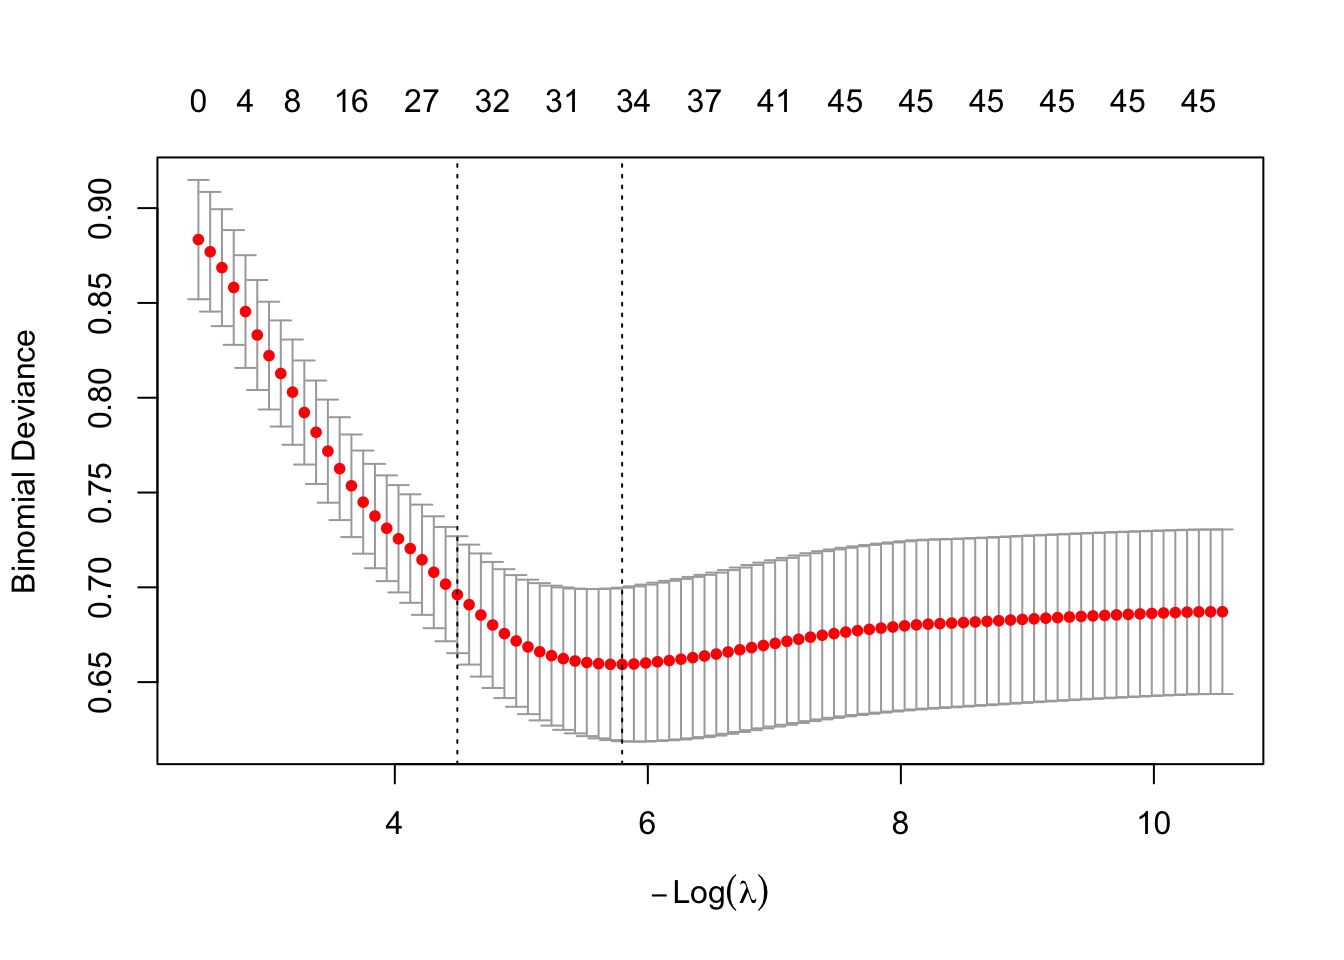
\includegraphics[width=0.82\linewidth]{img/hr-lasso-cv.png}
\caption{Sai số kiểm định chéo của mô hình LASSO theo tham số phạt.}
\label{fig:hr-lasso-cv}
\end{figure}

Khi \(\lambda\) tăng, hình phạt mạnh hơn và số hệ số khác 0 giảm. Hình
\ref{fig:hr-lasso-cv} thể hiện hai lựa chọn thường dùng:
\(\lambda_{\min}\), ưu tiên sai số CV nhỏ nhất và giữ 35 hệ số khác 0;
và \(\lambda_{1se}\), chọn mô hình đơn giản nhất còn nằm trong một sai số
chuẩn của cực tiểu, giữ 29 hệ số khác 0. Phân tích nguồn dùng
\(\lambda_{\min}\) để ưu tiên năng lực dự báo. Nếu ưu tiên triển khai
gọn, ít biến và ổn định hơn, \(\lambda_{1se}\) là đối chứng cần báo cáo.

\subsection{Đánh giá và lựa chọn mô hình}

\subsubsection{Kiểm tra giả định và giới hạn suy luận}

Biến phản hồi nhị phân đáp ứng yêu cầu của logistic. Các GVIF không cho
thấy đa cộng tuyến nghiêm trọng sau khi bỏ \texttt{Department}. Tuy
nhiên, tính độc lập của quan sát không thể khẳng định chỉ vì mỗi dòng là
một nhân viên; nếu nhiều nhân viên cùng nhóm hoặc quản lý, có thể tồn tại
phụ thuộc cụm. LASSO cũng không tự động bảo đảm quan hệ tuyến tính giữa
biến liên tục và log-odds. Quan hệ này nên được kiểm tra bằng
Box--Tidwell, spline, GAM hoặc binned residual plot. Các kiểm tra
calibration, Brier score và calibration curve chưa được báo cáo, nên AUC
tốt chưa đồng nghĩa xác suất dự báo đã được hiệu chỉnh tốt
\cite{hosmer2013,steyerberg2010}.

\subsubsection{Thước đo và ngưỡng phân loại}

AUC đánh giá khả năng xếp hạng ở mọi ngưỡng; accuracy đo tỷ lệ dự báo
đúng; sensitivity đo tỷ lệ phát hiện đúng người nghỉ việc; precision đo
tỷ lệ cảnh báo nghỉ việc thực sự đúng; và

\[
F_1=2\frac{\text{Precision}\times\text{Sensitivity}}
{\text{Precision}+\text{Sensitivity}}.
\]

Ngưỡng 0,3 được dùng thay cho 0,5 nhằm tăng sensitivity trong bối cảnh
lớp nghỉ việc chỉ chiếm 16,1\%. Đây là lựa chọn vận hành trung gian:
false negative (bỏ sót người sắp nghỉ) được xem là tốn kém hơn false
positive (mời một người ít rủi ro vào trao đổi giữ chân). Phần tối ưu
ngưỡng ở Mục \ref{sec:hr-threshold} cho thấy không có một ngưỡng duy
nhất tối ưu cho mọi tiêu chí.

\subsubsection{Kết quả so sánh}

\begin{table}[H]
\centering
\caption{Hiệu suất ba mô hình chính trên tập kiểm thử, ngưỡng 0,3.}
\label{tab:hr-main-comparison}
\begin{tabular}{lrrrr}
\toprule
Mô hình & AIC & AUC & Accuracy & Sensitivity\\
\midrule
Nhân khẩu học & 858,887 & 0,656 & 0,809 & 0,197\\
Công việc--môi trường & 781,322 & 0,785 & 0,818 & 0,465\\
LASSO toàn bộ biến & -- & 0,854 & 0,866 & 0,648\\
\bottomrule
\end{tabular}
\end{table}

Các chỉ số trong Bảng \ref{tab:hr-main-comparison} được diễn giải như
sau:

\begin{itemize}
  \item \textbf{AIC (Akaike Information Criterion)} được xác định bởi
  \[
    AIC=-2\log(\widehat{L})+2k,
  \]
  trong đó \(\widehat{L}\) là giá trị hợp lý cực đại và \(k\) là số tham
  số ước lượng. Thành phần thứ nhất đánh giá mức độ phù hợp với dữ liệu,
  còn \(2k\) phạt mô hình quá phức tạp. Vì vậy, \emph{AIC càng thấp càng
  tốt}, nhưng chỉ được so sánh giữa các mô hình ước lượng trên cùng tập
  dữ liệu và cùng biến phản hồi. AIC của mô hình công việc--môi trường
  thấp hơn mô hình nhân khẩu học \(77{,}565\) đơn vị, cung cấp bằng chứng
  rằng phần cải thiện độ phù hợp lớn hơn chi phí do bổ sung tham số.
  LASSO được ghi \texttt{--} vì hàm mục tiêu có hình phạt \(L_1\), nên
  AIC truyền thống không được xuất trực tiếp; mô hình này được chọn
  \(\lambda\) bằng kiểm định chéo.

  \item \textbf{AUC (Area Under the ROC Curve)} đo khả năng xếp hạng:
  xác suất mô hình gán điểm rủi ro cao hơn cho một nhân viên nghỉ việc
  so với một nhân viên ở lại được chọn ngẫu nhiên. AUC bằng 0,5 tương
  đương xếp hạng ngẫu nhiên, còn AUC bằng 1 biểu thị phân biệt hoàn hảo.
  Chỉ số này tổng hợp trên mọi ngưỡng, nên phù hợp để so sánh năng lực
  phân biệt tổng quát nhưng không cho biết trực tiếp hiệu quả tại ngưỡng
  vận hành 0,3.

  \item \textbf{Accuracy} là tỷ lệ dự báo đúng trên toàn bộ tập kiểm thử,
  \[
    \mathrm{Accuracy}=\frac{TP+TN}{TP+TN+FP+FN}.
  \]
  Giá trị 0,866 của LASSO nghĩa là mô hình phân loại đúng khoảng 86,6\%
  nhân viên kiểm thử tại ngưỡng 0,3. Tuy nhiên, do 83,88\% nhân viên
  thuộc lớp ở lại, accuracy cao vẫn có thể xuất hiện khi mô hình chủ yếu
  dự báo lớp đa số; vì vậy phải đọc cùng sensitivity.

  \item \textbf{Sensitivity (recall của lớp nghỉ việc)} là tỷ lệ nhân
  viên thực sự nghỉ việc được mô hình phát hiện,
  \[
    \mathrm{Sensitivity}=\frac{TP}{TP+FN}.
  \]
  Sensitivity 0,648 của LASSO nghĩa là mô hình nhận diện được 64,8\% số
  ca nghỉ việc và bỏ sót 35,2\%. Trong bài toán cảnh báo sớm, đây là chỉ
  số đặc biệt quan trọng vì false negative tương ứng với nhân viên có
  nguy cơ nhưng không được đưa vào diện xem xét can thiệp.
\end{itemize}

Mô hình nhân khẩu học có AUC 0,656 và chỉ phát hiện 19,7\% ca nghỉ việc;
accuracy 80,9\% còn thấp hơn baseline luôn dự báo ở lại 83,88\%. Mô
hình công việc nâng AUC lên 0,785 và sensitivity lên 46,5\%, cho thấy
trải nghiệm công việc chứa nhiều tín hiệu hơn nhân khẩu học. LASSO đạt
AUC 0,854, accuracy 86,6\% và sensitivity 64,8\%; đây là mô hình duy
nhất vượt baseline accuracy đồng thời có khả năng phát hiện lớp thiểu số
tốt nhất trong ba mô hình chính.

\begin{figure}[H]
\centering
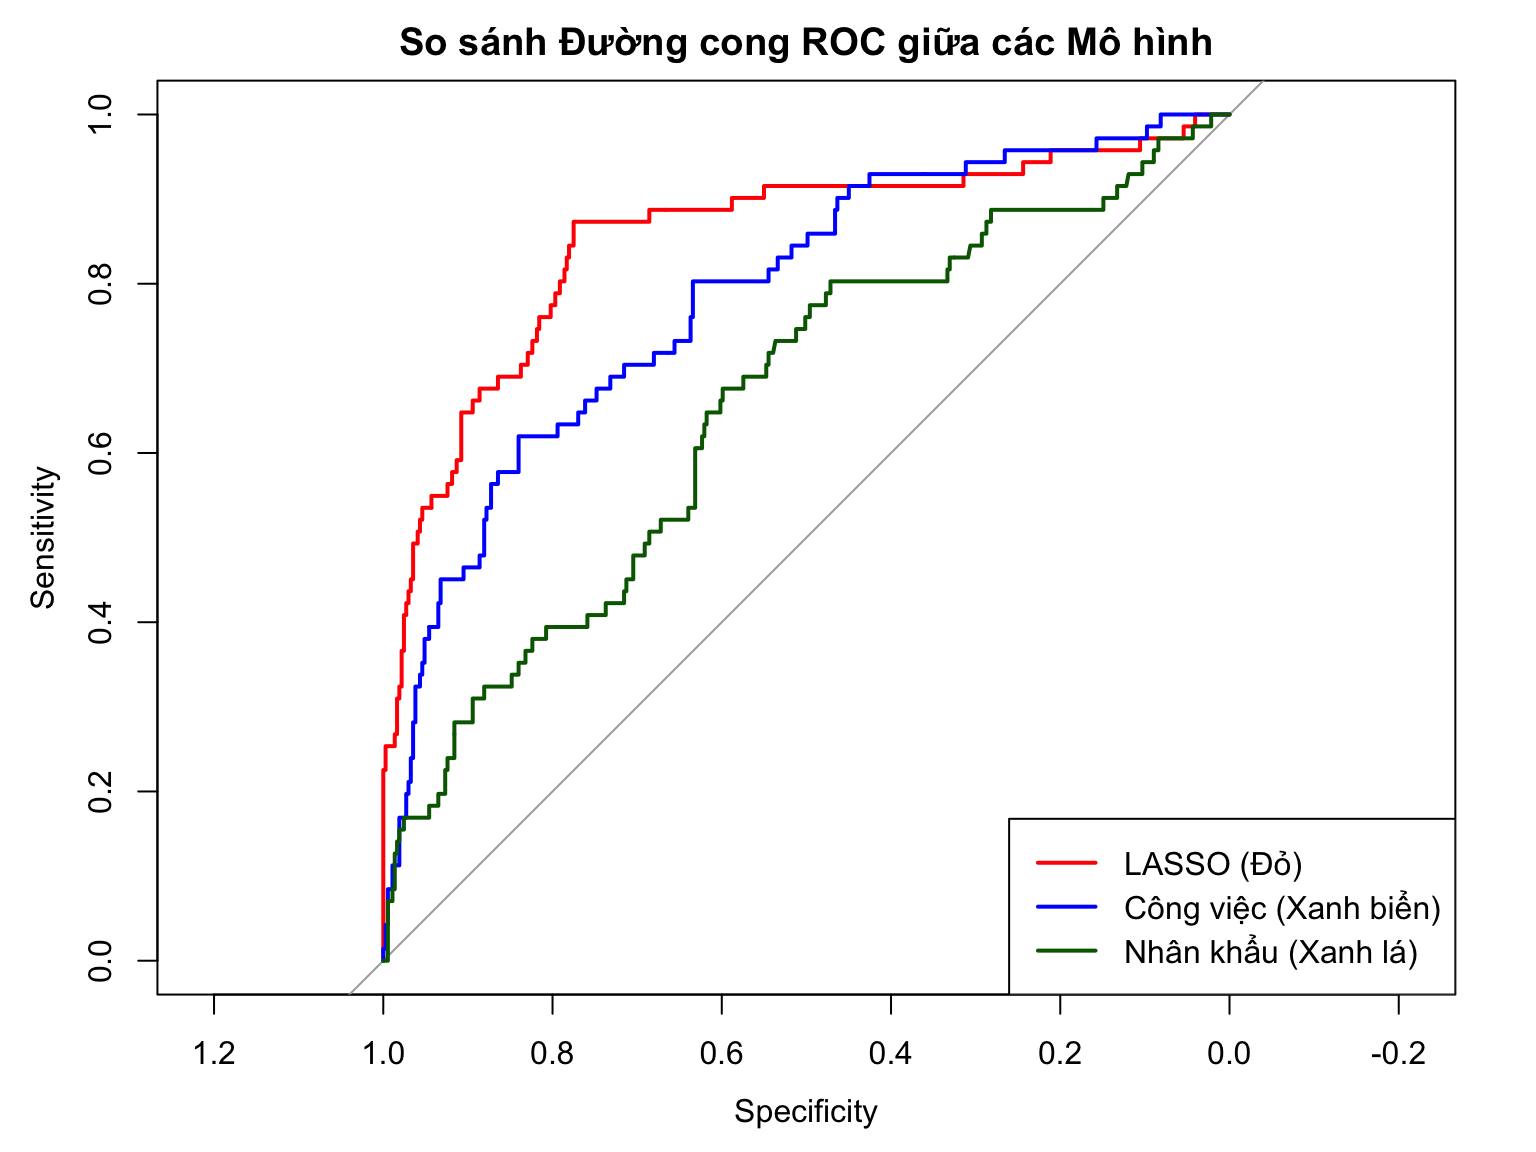
\includegraphics[width=0.82\linewidth]{img/hr-roc-logistic-models.png}
\caption{Đường cong ROC của ba mô hình chính.}
\label{fig:hr-roc-main}
\end{figure}

Đường ROC LASSO nằm nhìn chung phía trên hai đường còn lại, tiếp theo là
mô hình công việc và mô hình nhân khẩu học. Không nên suy ra sensitivity
tại ngưỡng 0,3 bằng cách đọc một điểm bất kỳ trên đường cong: mỗi điểm
ROC tương ứng một ngưỡng khác nhau. Vì vậy, sensitivity 64,8\% trong
Bảng \ref{tab:hr-main-comparison} là kết quả vận hành tại ngưỡng 0,3,
còn AUC 0,854 là kết quả tổng hợp trên mọi ngưỡng.

\subsubsection{Tối ưu hóa và lựa chọn ngưỡng quyết định}
\label{sec:hr-threshold}

Phiên bản báo cáo mới khảo sát các ngưỡng từ 0,05 đến 0,80 theo ba tiêu
chí. Thứ nhất, ngưỡng tối đa hóa F1 là 0,30 với
\(F1_{\max}=0,609\). Thứ hai, chỉ số Youden
\(J=\text{Sensitivity}+\text{Specificity}-1\) chọn ngưỡng 0,17. Thứ
ba, với giả định chi phí một false negative là 15.000 USD và một false
positive là 1.000 USD, hàm

\[
C(t)=15.000\,FN(t)+1.000\,FP(t)
\]

cũng đạt cực tiểu tại ngưỡng 0,17.

\begin{table}[H]
\centering
\caption{Các ngưỡng đề xuất theo từng tiêu chí.}
\label{tab:hr-thresholds}
\begin{tabular}{lcc}
\toprule
Tiêu chí & Ngưỡng đề xuất & Ý nghĩa\\
\midrule
F1-score & 0,30 & Cân bằng precision và recall\\
Youden's J & 0,17 & Cân bằng sensitivity và specificity\\
Chi phí giả định & 0,17 & Ưu tiên tránh false negative đắt đỏ\\
Ngưỡng vận hành & 0,30 & Ưu tiên F1 và duy trì độ nhạy 64,8\%\\
\bottomrule
\end{tabular}
\end{table}

\begin{figure}[H]
\centering
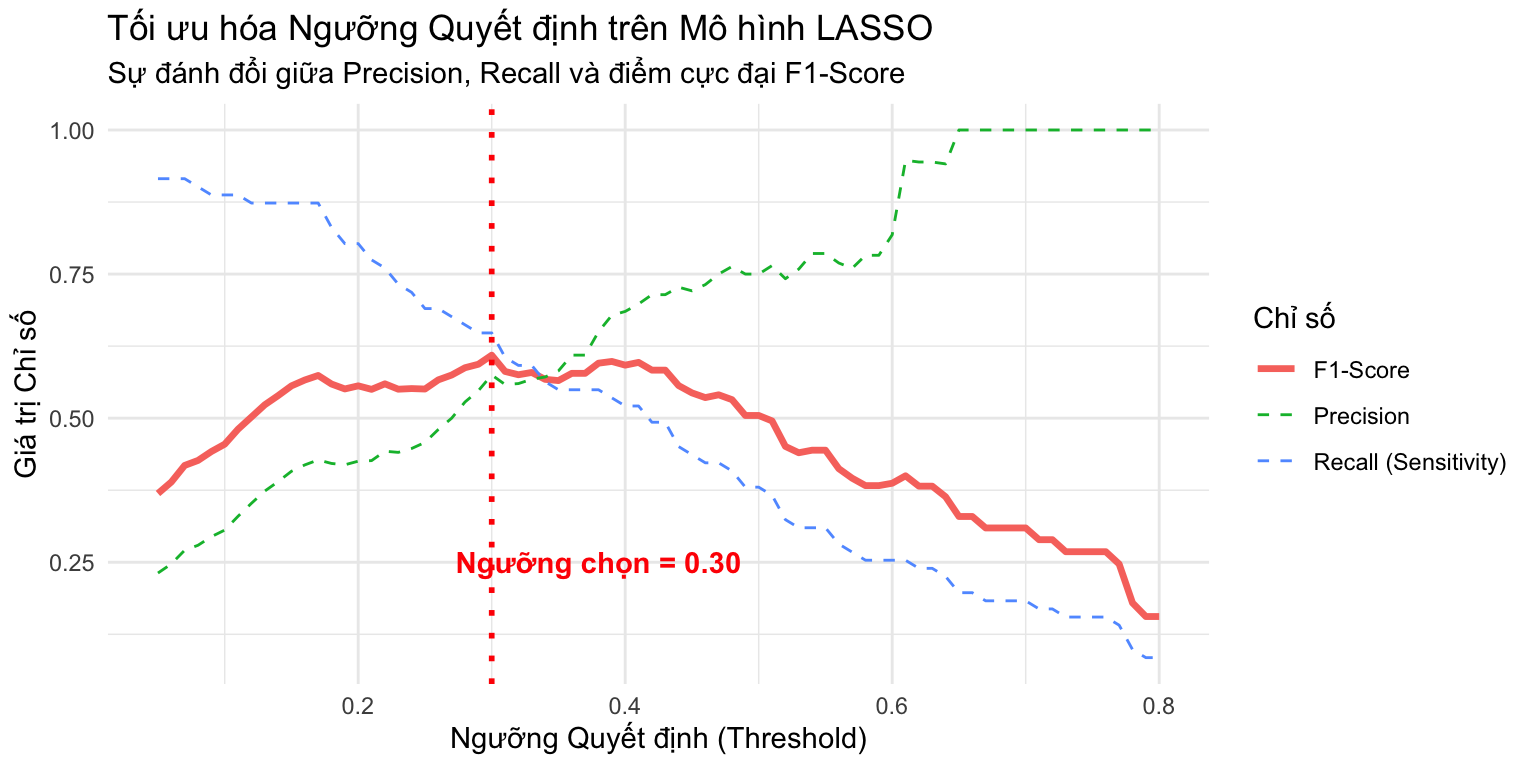
\includegraphics[width=0.88\linewidth]{img/hr-threshold-optimization.png}
\caption{Precision, recall và F1 của LASSO theo ngưỡng quyết định.}
\label{fig:hr-threshold-optimization}
\end{figure}

Không có một ngưỡng tối ưu đồng thời cho mọi mục tiêu: F1 chọn 0,30,
còn Youden và hàm chi phí giả định chọn 0,17. Ở ngưỡng 0,30, LASSO phát
hiện 64,8\% ca nghỉ việc, đạt specificity khoảng 90,8\% và giới hạn tỷ
lệ cảnh báo giả ở khoảng 9,2\%. Vì vậy, 0,30 phù hợp cho kịch bản vận
hành cân bằng; ngưỡng 0,17 phù hợp hơn khi chi phí bỏ sót được xem là
rất cao. Các ngưỡng trên được tìm trực tiếp trên tập test;
nếu tiếp tục dùng chính tập này để báo cáo hiệu suất cuối, tập test đã
trở thành tập validation. Quy trình chặt chẽ hơn cần chọn ngưỡng trong
cross-validation của tập train hoặc trên validation riêng, rồi chỉ đánh
giá một lần trên test độc lập.

\subsubsection{Lựa chọn mô hình và diễn giải quyết định}

Trong ba mô hình chính, LASSO có AUC 0,854, accuracy 86,6\% và
sensitivity 64,8\%, đều cao hơn hai mô hình logistic theo nhóm biến.
Do đó, \textbf{LASSO logistic được chọn làm mô hình vận hành chính} vì:

\begin{enumerate}
  \item có AUC và khả năng phát hiện lớp nghỉ việc cao nhất tại ngưỡng
  vận hành 0,3;
  \item cho phép giải thích chiều tác động và odds ratio, phù hợp yêu
  cầu minh bạch của quyết định nhân sự;
  \item co rút và chọn biến, giảm nguy cơ quá khớp so với logistic đầy
  đủ;
  \item triển khai, giám sát và hiệu chỉnh thuận lợi trong quy trình HR.
\end{enumerate}

Quyết định cuối cùng không dựa riêng AUC mà còn dựa trên mục tiêu, chi
phí lỗi, độ ổn định và yêu cầu giải thích \cite{fawcett2006}.

\subsection{Phân tích và diễn giải kết quả}

\subsubsection{Các yếu tố liên hệ với rủi ro nghỉ việc}

Kết quả thống nhất cho thấy các biến bối cảnh công việc có giá trị dự
báo lớn hơn nhóm nhân khẩu học đơn thuần. Làm thêm giờ là tín hiệu nổi
bật: odds nghỉ việc cao khoảng 4,67 lần trong mô hình công việc. Mức hài
lòng môi trường và công việc tăng một bậc liên hệ với odds giảm lần lượt
khoảng 30,3\% và 24,8\%. Laboratory Technician, Sales Representative,
Sales Executive và Human Resources là các chức danh cần được theo dõi;
tuy nhiên, odds ratio phụ thuộc nhóm tham chiếu và không nên diễn giải
như rủi ro tuyệt đối.

Nhân viên trẻ, độc thân và ở xa nơi làm việc cũng có rủi ro dự báo cao
hơn. Nhân viên độc thân có odds cao khoảng 2,47 lần nhóm đã ly hôn trong
mô hình nhân khẩu học; mỗi đơn vị khoảng cách liên hệ với odds tăng
3,1\%. EDA cho thấy chân dung rủi ro thường nằm ở tuổi 28--32, thu nhập
dưới khoảng 5.000 USD/tháng, làm việc tại Sales hoặc R\&D và thường làm
thêm giờ. Đây là hồ sơ mô tả để ưu tiên khảo sát, không phải quy tắc tự
động ra quyết định bất lợi đối với cá nhân.

\subsubsection{Mức độ hoàn thành mục tiêu và hàm ý quản trị}

Mục tiêu khám phá dữ liệu được đáp ứng qua việc nhận diện nhóm nhân viên
trẻ, thu nhập thấp, làm thêm giờ và thuộc một số chức danh có tỷ lệ nghỉ
việc cao hơn. Mục tiêu dự báo được đáp ứng bằng việc xây dựng ba mô hình,
đánh giá ngoài mẫu và lựa chọn LASSO. Mục tiêu quản trị được chuyển hóa
thành các hành động ưu tiên dưới đây; các hành động tập trung vào yếu tố
có thể can thiệp thay vì dùng đặc điểm cá nhân để tự động ra quyết định.

\begin{itemize}
  \item \textbf{Kiểm soát làm thêm giờ:} theo dõi số giờ OT theo nhóm,
  phân bổ lại tải công việc, yêu cầu quản lý giải trình các đợt OT kéo
  dài và đo lường kiệt sức định kỳ.
  \item \textbf{Can thiệp theo chức danh:} thực hiện khảo sát ẩn danh và
  \emph{stay interview} với Laboratory Technician, Sales Representative
  và Sales Executive để xác định vấn đề về tải việc, đãi ngộ và lộ trình
  nghề nghiệp.
  \item \textbf{Nâng chất lượng trải nghiệm:} theo dõi điểm hài lòng
  môi trường/công việc theo thời gian, gắn phản hồi với kế hoạch cải thiện
  của quản lý trực tiếp.
  \item \textbf{Chính sách linh hoạt cho nhân sự trẻ và độc thân:} hỗ
  trợ đào tạo, luân chuyển nội bộ, lộ trình thăng tiến rõ ràng, phúc lợi
  tự chọn và trợ cấp đi lại thay cho một gói phúc lợi đồng nhất.
  \item \textbf{Hệ thống cảnh báo sớm:} chấm điểm hàng tháng bằng LASSO.
  Có thể dùng hai tầng: từ 0,17 để theo dõi rộng khi chi phí bỏ sót cao
  và từ 0,30 để HR rà soát, trao đổi 1--1 theo tiêu chí F1. Các ngưỡng
  phải được hiệu chỉnh lại trên dữ liệu vận hành, không kích hoạt quyết
  định kỷ luật hay sa thải tự động.
\end{itemize}

Mô hình phải được dùng như công cụ hỗ trợ, không phải cơ chế quyết định
duy nhất. Các thuộc tính nhạy cảm như giới tính, tuổi và tình trạng hôn
nhân cần được kiểm tra fairness, quyền riêng tư và tính hợp pháp trước
khi triển khai. Tốt hơn nên ưu tiên các biến có thể can thiệp như tải
việc, hài lòng và cơ hội phát triển.

\subsection{Đề xuất và kết luận}

\subsubsection{Hướng cải thiện dữ liệu và mô hình}

\begin{enumerate}
  \item \textbf{Tính đại diện:} dữ liệu là mô phỏng và chỉ phản ánh một
  lát cắt; chưa có thời gian nghỉ việc, kiểm duyệt hay biến động theo
  chu kỳ kinh tế. Cần kiểm định ngoài mẫu trên dữ liệu thực tế.
  \item \textbf{Pipeline và lựa chọn siêu tham số:} phiên bản mới đã fit
  capping, chuẩn hóa và dummy encoding trên train. Tuy nhiên,
  \(\lambda\), cấu hình mô hình và đặc biệt ngưỡng quyết định vẫn nên
  được chọn trong nested cross-validation; tập test chỉ dùng một lần.
  \item \textbf{Ngoại lệ thu nhập:} so sánh mô hình dùng thu nhập gốc,
  log-thu nhập, spline và winsor hóa; không capping chỉ vì vượt quy tắc
  IQR.
  \item \textbf{Mất cân bằng lớp:} thử trọng số lớp, SMOTE hoặc ROSE chỉ
  trong từng fold huấn luyện để tránh leakage \cite{chawla2002}; so sánh
  thêm PR-AUC vì lớp dương hiếm.
  \item \textbf{Ngưỡng quyết định:} các kết quả 0,17 và 0,30 phụ
  thuộc tiêu chí và giả định chi phí. Cần ước lượng chi phí false negative
  và false positive từ dữ liệu doanh nghiệp, đồng thời kiểm tra độ nhạy
  khi tỷ lệ chi phí thay đổi.
  \item \textbf{Quan hệ phi tuyến và tương tác:} kiểm tra spline/GAM,
  Elastic Net, Random Forest, GBDT/XGBoost với tuning có hệ thống. Ví dụ,
  tác động của thu nhập có thể phụ thuộc mức hài lòng hoặc chức danh.
  \item \textbf{Hiệu chỉnh và độ ổn định:} báo cáo Brier score,
  calibration intercept/slope, khoảng tin cậy bootstrap cho AUC và độ
  ổn định chọn biến LASSO.
  \item \textbf{Mở rộng đặc trưng:} bổ sung lịch sử tăng lương, nghỉ ốm,
  biến động điểm hài lòng, khối lượng công việc, thăng tiến, phản hồi văn
  hóa và dữ liệu quản lý. Việc dùng dữ liệu mạng xã hội nghề nghiệp chỉ
  nên cân nhắc khi có cơ sở pháp lý, đồng thuận và đánh giá quyền riêng tư.
\end{enumerate}

\subsubsection{Kết luận}

Phân tích đã hoàn thành ba mục tiêu: nhận diện các tín hiệu liên hệ với
nghỉ việc, xây dựng và so sánh các mô hình dự báo, và chuyển kết quả
thành khuyến nghị nhân sự. Mô hình nhân khẩu học có sức dự báo yếu; mô
hình công việc cải thiện rõ rệt; LASSO logistic đạt AUC 0,854,
accuracy 86,6\%, sensitivity 64,8\%, precision 57,5\% và F1 0,609 tại
ngưỡng 0,3. LASSO được chọn cho mục tiêu cảnh báo sớm nhờ sự cân bằng
giữa hiệu suất, khả năng giải thích và tính triển khai.

Kết quả quan trọng nhất về quản trị không phải là gắn nhãn cá nhân, mà
là chuyển trọng tâm từ đặc điểm cố định sang các điều kiện có thể cải
thiện: làm thêm giờ, trải nghiệm công việc, sự hài lòng, cơ hội phát
triển và chính sách theo chức danh. Trước khi vận hành thực tế, cần tái
duy trì pipeline không rò rỉ, chọn ngưỡng trong validation hoặc nested
CV, đánh giá calibration/fairness và xác nhận hiệu suất trên dữ liệu
doanh nghiệp.

\subsection{Mở rộng nghiên cứu với mô hình phi tuyến}

Để kiểm tra liệu quan hệ phi tuyến và tương tác có cải thiện dự báo,
báo cáo thử thêm Random Forest và Gradient Boosting Decision Trees
(GBDT). Random Forest dùng 300 cây, \texttt{nodesize=5} và trọng số lớp
\(1:5\) cho \texttt{No:Yes}. GBDT dùng 150 cây, độ sâu tương tác 3,
learning rate 0,05 và 5-fold cross-validation. Hai mô hình được đánh giá
trên cùng tập kiểm thử và tại ngưỡng 0,3 để bảo đảm khả năng so sánh.

\begin{table}[H]
\centering
\small
\caption{So sánh LASSO và hai mô hình phi tuyến, ngưỡng 0,3.}
\label{tab:hr-advanced-comparison}
\begin{tabular}{lrrrrr}
\toprule
Mô hình & AUC & Accuracy & Sensitivity & Precision & F1\\
\midrule
LASSO logistic & 0,854 & 0,866 & 0,648 & 0,575 & 0,609\\
Random Forest cân bằng & 0,802 & 0,818 & 0,507 & 0,444 & 0,474\\
GBDT & 0,841 & 0,859 & 0,465 & 0,579 & 0,516\\
\bottomrule
\end{tabular}
\end{table}

LASSO tiếp tục có AUC, accuracy, sensitivity và F1 cao nhất. GBDT có
precision cao nhất nhưng chỉ nhỉnh hơn LASSO 0,004, trong khi
sensitivity thấp hơn 18,3 điểm phần trăm. Random Forest cân bằng bắt
được nhiều ca nghỉ việc hơn GBDT nhưng tạo nhiều cảnh báo giả hơn. Vì
mục tiêu chính là cảnh báo sớm và hạn chế bỏ sót, kết quả mở rộng không
làm thay đổi lựa chọn LASSO. Tuy nhiên, chưa thể kết luận các thuật toán
cây nói chung không phù hợp, do mỗi mô hình mới sử dụng một cấu hình và
chưa được tối ưu bằng nested cross-validation.

\begin{figure}[H]
\centering
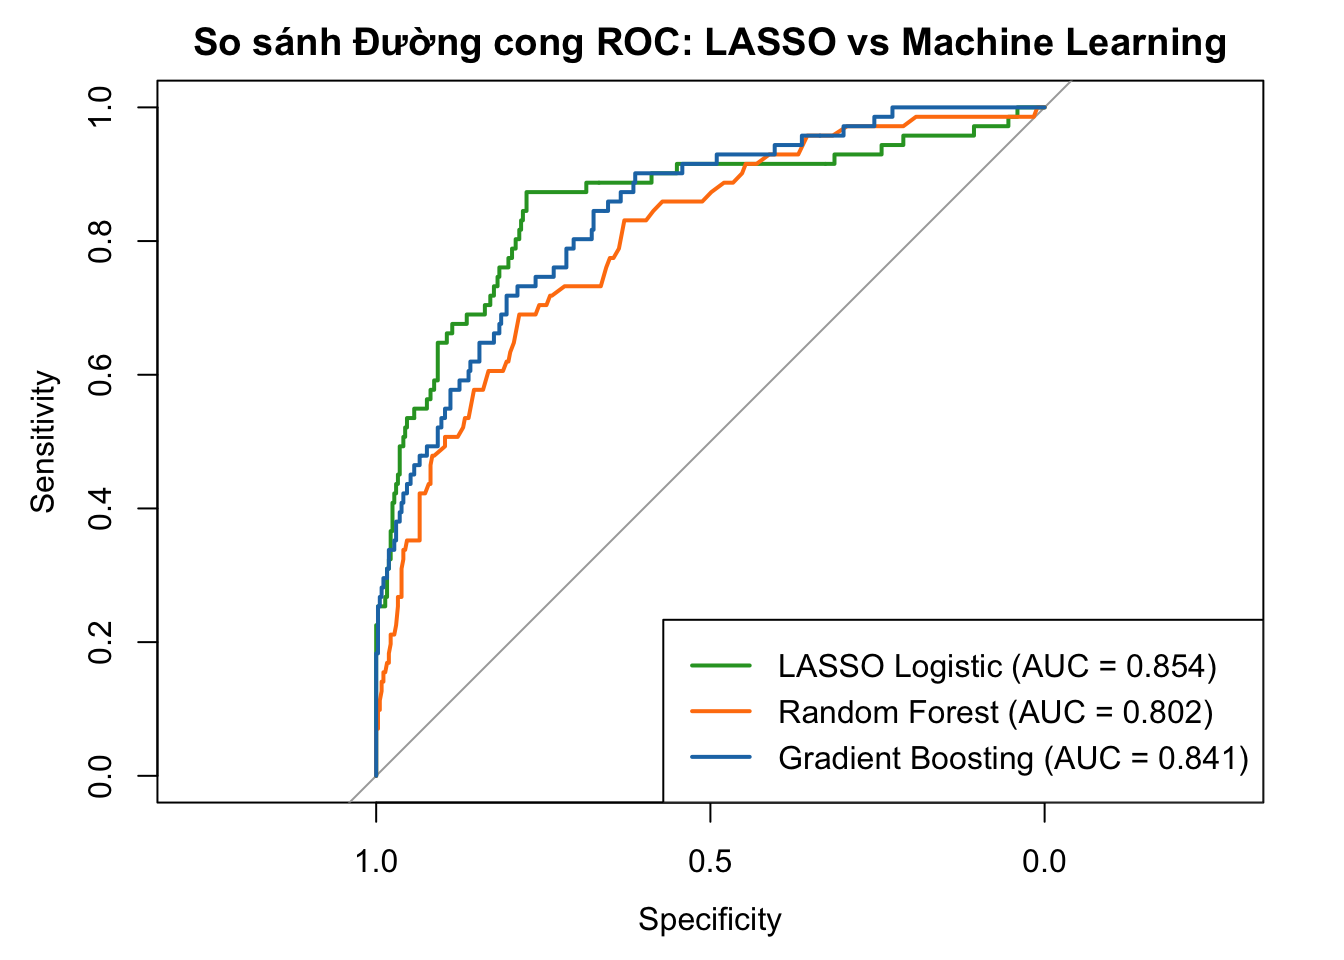
\includegraphics[width=0.82\linewidth]{img/hr-roc-advanced-models.png}
\caption{Đường ROC trong thử nghiệm LASSO, Random Forest và GBDT.}
\label{fig:hr-roc-advanced}
\end{figure}

Phần mở rộng được đặt sau kết luận chính theo cấu trúc của báo cáo nguồn:
ba mô hình logistic trả lời trực tiếp câu hỏi nghiên cứu, còn Random
Forest và GBDT đóng vai trò kiểm tra độ bền của quyết định lựa chọn mô
hình. Trong triển khai thực tế, chúng có thể được duy trì như mô hình đối
chứng để phát hiện suy giảm hiệu suất hoặc thay đổi cấu trúc dữ liệu theo
thời gian.
